%!TEX root = Main.tex
% System testing: words
\chapter{System Testing and Results} % (fold)
\label{cha:system_testing}

% Screenshots of data being sent and received (Logic)
% SystemVerilog simulations in ModelSim
% Hardware vs Software timing??? Roughly???
% Timing analysis / diagrams
% TODO: do some hardware analysis - how much current draw etc?

The testing methods and results are documented in this chapter, along with an analysis of the final design.  The two primary blocks, described in the last chapter, were tested independently and then together, and will be presented here in the same manner.  A wide range of tools and techniques have been used to perform the testing, and to identify and fix errors encountered.

% Testing & things to document:
% x Testing methodology
% x GDP (software & hardware)
% x UART
% x SRAM (pre-tests, etc)
% MFCCs
% Time of calculations, hardware vs software
% Full System - bus pirate, etc
% Hardware testing?? Current draw etc? .... Nah

\section{FPGA Design and Test methodology} % (fold)
\label{sec:fpga_design_and_test_methodology}
	There were several phases of development, and thus testing, of this part of the design.  Initially, the full system was written and simulated in ModelSim, which supports SystemVerilog assertion based verification.  Each of the components of the design was built and tested separately, and then incrementally joined together and simulated as a whole.  Finally, the modules were tested in hardware -- first individually, and then as a full system.

	A set of testbenches were developed for use within ModelSim, which tested each of the modules used by the system.  Most of the modules were fairly simple to simulate and verify, as the expected behaviour is generally constant and determinate.  For example, verifying the UART clock generator was a case of instantiating it, asserting the enable signal, and verifying the frequency of the output signals.  However, some modules and their testbenches deserve extra attention, as special methods were used to test them.  In several areas, the benefits of using SystemVerilog become clear, as assertions greatly simplified the validation and testing process.
% section fpga_design_and_test_methodology (end)


\section{Gaussian Distance Calculation Block} % (fold)
\label{sec:gaussian_distance_calculation_testing}
	The Gaussian Distance Pipe was initially tested by creating a testbench which provided the sequence of inputs that the GDP required, and then asserted that the correct score was provided.  Figure~\ref{fig:test_gdp} shows the correct operation of this module, with a set of test data being used as inputs to the module.  The expected results were determined using the software GDP and the binary conversion software described in Section~\ref{sec:support_software}, thus confirming the validity of the results produced.

	\begin{figure}[tb]
		\begin{center}
			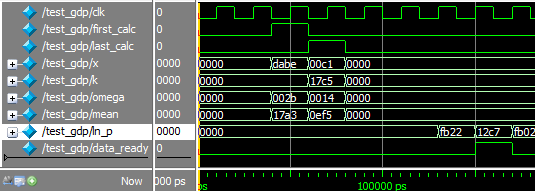
\includegraphics[width=\figwidth]{testbenches/gdp_wave.png}
		\end{center}
		\caption{GDP testbench waveform}
		\label{fig:test_gdp}
	\end{figure}
	
	The Gaussian Distance pipe controller testbench gives a new observation to the controller, and then watches as senone scores are produced by the module.  SystemVerilog assertions are used to check whether correct scores are arriving at the time they should.  However, in order to test a large number of different inputs (which would result in different score outputs), a set of software utilities were written to automatically generate the testbench code.  This software made use of the HMM definition parser and a software version of the GDP that had already been created.  This allowed a very large number of senones to be tested in a matter of minutes, and determine how well the GDP pipe was working.  Figure~\ref{fig:test_gdp_ctrl} shows the GDP Controller being tested, with an example of the type of error message used to examine its behaviour.  In this test, % TODO: x of y senones had z error..

	Being able to easily test many senones was important because the use of fixed-point arithmetic inevitably causes numerical errors that vary with the operations and numbers being used.  The GDP may produce the correct result for one set of inputs, but another set of inputs may produce an erroneous result that was caused by the fixed-point number not having high enough precision.  In fact, in most cases, the least significant bits of the result were usually wrong.  Because of this, it was important to determine the distribution of the error magnitudes, in order to decide whether the number format needed changing.  Automatic testbench generation made this far easier, as testbenches could be created which automatically displayed which senone scores where wrong, and by how much.

	% TODO: talk about the error distribution??? I speak lots about how I found it (^) but don't actually say what the results were...

	\begin{figure}[tb]
		\begin{center}
			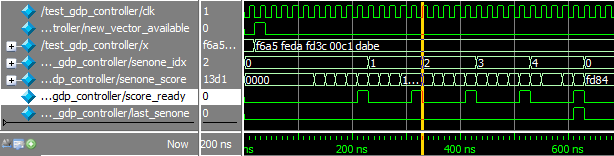
\includegraphics[width=\figwidth]{testbenches/gdp_ctrl_wave.png}
		\end{center}
		\caption{GDP Controller testbench waveform and error messages}
		\label{fig:test_gdp_ctrl}
	\end{figure}

	\subsection{Synthesis and Hardware Testing} % (fold)
	\label{sub:gdp_synthesis_and_hardware_testing}
		Unfortunately, due to the small size of the FPGA used, the initial synthesised design did not fit on it.  The full Voxforge model had over 7000 senones, and each observation had 25 parameters of 2 bytes each -- over 700kB of storage would be required for the full model.  As this far exceeds the resources available, the model size was reduced for this proof-of-concept project.  The number of statistical parameters was reduced to 6, and only 3 senones were scored at once, bringing the total resource usage to about 90\%.  % TODO: confirm this

		A variety of tools were used to repeatedly test the functionality of this hardware.  A Bus Pirate\footnote{Multi-purpose debugging tool that supports many different protocols.  See \href{http://dangerousprototypes.com/docs/Bus_Pirate}{http://dangerousprototypes.com/docs/Bus_Pirate}} was used to communicate with the FPGA, which allows hexadecimal values to be easily sent and received over UART.  In order to debug the SystemVerilog, a large number of signals were routed to pins on the FPGA, which were then monitored with a Saleae Logic analyser.

		% TODO: test the calc speed
	% subsection gdp_synthesis_and_hardware_testing (end)
% section gaussian_distance_calculation_testing (end)


\section{UART communications} % (fold)
\label{sec:uart_communications_testing}
	Simulating and testing the UART module was done by creating two instances of the module, and cross-connecting their RX and TX pins.  This allowed both transmit and receive to be tested, and confirmed correct operation.  An example of this testbench running is shown in Figure~\ref{fig:test_uart}.  

	\begin{figure}[tb]
		\begin{center}
			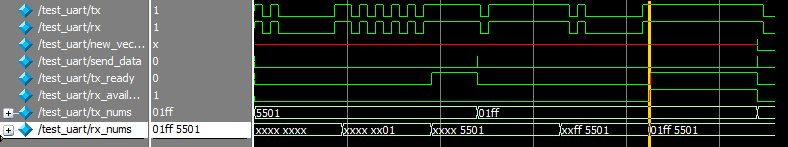
\includegraphics[width=\figwidth]{testbenches/uart_wave.png}
		\end{center}
		\caption{UART testbench waveform}
		\label{fig:test_uart}
	\end{figure}

	After simulation, the UART module was finally verified by programming the FPGA with the UART module, and a simple controller which echoed back whatever it received.  An FTDI USB to serial cable connected the FPGA to a computer, so that the setup could be confirmed to work with a real UART connection.  In addition, a Saleae Logic analyser was used to examine and ensure the absence of glitches in the UART signals generated by the FPGA.
% section uart_communications_testing (end)


\section{SRAM access} % (fold)
\label{sec:sram_access_testing}
	A custom SystemVerilog module was designed in order to test writing and reading values to the onboard SRAM chip, as it was a completely untested part of the board.  The module performed fairly basic operations, such as looping through a set of values, writing them to SRAM, and then reading them out again.  Debug information was displayed on the output pins, allowing the process to be monitored.  This confirmed that the chip worked as expected, and would be usable for the project.
% section sram_access_testing (end)


\section{Pre-Processing} % (fold)
\label{sec:pre_processing_testing}
	There were several different stages to the pre-processing, and these were tested individually.  First and foremost, the FFT code was tested by using, as input data, a set of data containing known sinusoidals.  The library used, FFTW, is well established and proven to work, and so the primary purpose here was to test the speed of the FFT.  It ran almost instantaneously (execution took 0.00000s, according to the Kernel time.h library), giving the correct results. %TODO confirm this!

	The other major operation that required extensive testing was the MFCC calculation.  The other operations, pre-emphasis, windowing and liftering, are fairly simple mathematical operations that are easy to verify.  One of the desired properties of the system is that it would produce MFCCs that matched those produced by the HTK. Unfortunately, this was not quite acheived.  In most tests, the energy coefficients matched, but the others were relatively different.  This implies either that there is a limitation or problem with the MFCC library used, or that the HTK performs extra (or different) pre-processing.

	To be used in a real system, an important requirement is that all the pre-processing is much faster than the frame period.  With the current design, the only component breaking this requirement is the MFCC computation, due to the library's slowness and inefficiency.  All the other steps take a tiny fraction of the frame period, allowing a large amount of time for processing, and in later designs, decoding.
% section pre_processing_testing (end)


\section{Full system} % (fold)  % TODO
\label{sec:full_system_testing}
	Once all the separate modules were tested and verified, the final task was to identify and eliminate the inevitable errors that occur once a design is integrated.

% section full_system_testing (end)


% chapter system_testing (end)